\Chapter{A fejlesztőkörnyezet implementációja}

\graphicspath{{./kepek/}}

\Section{Minimális program: egy fájlt kezelő kódszerkesztő}

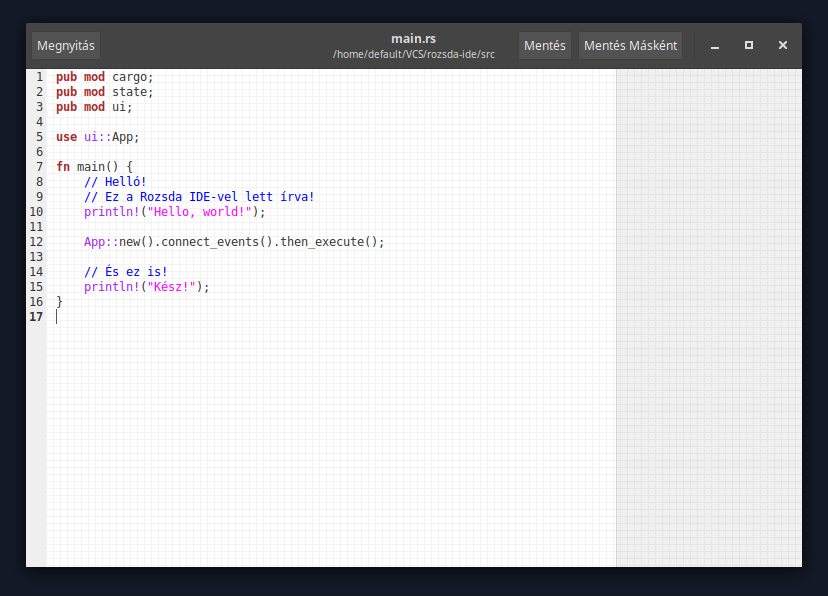
\includegraphics[width=\textwidth]{program-mvp}

A program implementációját egy olyan minimális életképes termék elkészítésével kezdjük,
ami meg tud nyitni egyszerre egy fájlt, annak tartalmát megfelelően dekorálja,
ha az egy Rust forráskód-fájl, és tud az eredeti, vagy egy másik megadott fájlba menteni.

A programnak ez a része Michael Murphy \textit{Simple Common Mark Editor} projektjén alapul.\cite{gtk_tutorial}
Murphy programra Markdown formátumú fájlokat kezel, illetve azokat HTML formátumra lefordítja,
és megjeleníti a felhasználónak.
A leglényegesebb változtatások ezen a programon a Markdown nyelv lecserélése a Rust nyelvre,
a projekt frissítése egyrészt a Rust 2018-as verziójára, illetve a függőségek frissítése a legújabb verziókra.

A projekt egy \texttt{cargo new} parancshívással kezdődik.

\SubSection{Cargo.TOML}

\lstinputlisting{./kodreszletek/01_cargo.toml}

A projekt Cargo.TOML-jában nincs semmi különös.
A \texttt{package} kategória legtöbb értéke nem lényeges, mivel ezeket a Cargo használja fel
a \url{crates.io}-ra való publikáláskor.
A mi szempontunkból az egyetlen kitűnő érték az az \texttt{edition}, amivel a Rust 2018-as
kiadásának használatát kérjük a \texttt{rustc}-től.
A 2015-ös és a 2018-as kiadás kompatibilis egymással,\cite{rust:editions}
a legnagyobb előnye a frissítésnek a programozás megkönnyítése az új nyelvi tulajdonságokkal.
A \texttt{dependencies} kategória leírja a projekt függőségeit, és a függőségek kötelező verziószámát.
Itt konkrét verziószámokat adtunk meg, de lehetőség van a Cargo-ra hagyni az optimális verziók kiderítését is.
A \texttt{GTK} és a \texttt{SourceView} esetén azt is megadjuk, 
hogy ezek a Rust könyvtárak az alattuk lévő könyvtárak melyik verziójára épüljenek rá
(a megadott \texttt{SourceView} Rust könyvtár verziószáma disztinkt a C-ben íródott \texttt{SourceView}
projekt verziószámától).

\SubSection{Az \texttt{App} és a \texttt{SourceView}}

\subsubsection{Az \texttt{ui} modul}

A felhasználói felülettel kapcsolatos forráskódokat az olvashatóság kedvéért egy modulba tesszük,
az \texttt{ui} modulba.
A modulkészítés a Rust 2018-as kiadásában forrásfájlokon alapul -- 
minden új forrásfájl egy új modult jelent (néhány kivétellel, mint például \texttt{build.rs}).
Egy modulnak adhatunk al-modulokat, ha létrehozunk a forrásfájlával megegyező nevű könyvtárat (fájlrendszer-entitás értelemben),
és azon belül hozunk létre új forrásfájlokat.

Így létrehozunk egy \texttt{ui.rs} forrásfájlt.

\lstinputlisting[firstline=4, lastline=8, language=Rust]{./kodreszletek/01_app.rs}

Ezt a forrásfájlt nem fogjuk új kód definiálására használni.
Két szerepe lesz, és a fenti kódrészletből mindkettő nyilvánvaló: 
egyszer definiál al-modulokat a \texttt{mod} kulcsszóval,
majd bizonyos struktúrákat elérhetővé tesz a \texttt{pub use} kombinációval.
A \texttt{use} kulcsszó behívja a megadott struktúrát és metódusait a forrásfájlba,
míg a \texttt{pub} nyilvánossá, azaz modulon kívül elérhetővé teszi a struktúrát.
Ezt \textit{újraexportálásnak} (re-export) hívják a Rust nyelvben.

\subsubsection{Az applikáció}

Következőnek az \texttt{ui/app.rs}-t hozzuk létre:

\lstinputlisting[firstline=13, lastline=42, language=Rust]{./kodreszletek/01_app.rs}

A Rust nyelvben egy struktúra adattagjai, és a struktúrán végezhető műveletek két külön blokkba
kerülnek: a \texttt{struct} és az \texttt{Impl} blokkokba.
Ez utóbbi szerepet játszik a tulajdonságok implementálásakor is.

Egyelőre egy metódust definiálunk, a \texttt{new()} metódust.
Ez a metódus statikus, nem egy példányra vonatkozik, hanem a típusra magára.
Egy metódus akkor vonatkozik egy példányra, ha annak első paramétere saját maga, vagy referencia saját magára
(\texttt{self} vagy \verb+&self+).

Legelső lépésként inicializáljuk a GTK rendszerét.
Ha az hibával tér vissza, akkor a standard hiba csatornán jelezzük azt, majd kilépünk a programból.
Ellenkező esetben létrehozzuk a GTK-s ablakot, illetve a \texttt{Content} struktúránkat,
beállítjuk az ablak nevét és méretét, majd visszatérünk az osztállyal.

A \verb+connect_delete_event()+ kitűnik, bár igazából az is magától értetődő.
A metódus egyetlen paraméternek egy másik metódust kér, ami egy \texttt{Inhibit} struktúrával tér vissza.
Ennek a paramétermetódusnak magának is egy paramétere kell, hogy legyen, egy referencia az eseményre.
Ezt a paramétermetódust helyben definiáljuk egy lexikai zárvány (closure) segítségével.
A \verb+move |_, _|+ kijelenti, hogy egy zárványt írunk le, és két (névtelen) paramétert adunk neki --
ne feledjük, hogy nem statikus metódusok esetén a tényleges első paraméter egy referencia a struktúrára magára!
Ennek ellenére a zárvány paraméterei névtelenek maradtak azért, mert nem használtuk fel őket magában a zárványban.

A zárvány tartalma ehhez képest egyszerű.
Meghívjuk a GTK rendszer kilépő metódusát, majd visszatérünk egy hamis értékű \texttt{Inhibit} struktúrapéldánnyal --
Nem kell a jelzést tovább küldeni, a programot már bezárásra késztettük.

\subsubsection{Az ablak fejléce}

A következő legegyszerűbb része a programnak a fejléc elkészítése.
A fejlécen fog szerepelni az első verziókban a \textit{Megnyitás,} \textit{Mentés,} és \textit{Mentés Másként}
gombok, továbbá a megnyitott fájl neve,
illetve a későbbiekben itt lesznek az általában elvárt \textit{Fájl,} \textit{Szerkesztés,} és egyéb menük.

Az újonnan elkészített \texttt{ui/header.rs} tartalma tehát a következő lesz:

\lstinputlisting[firstline=46, lastline=72, language=Rust]{./kodreszletek/01_app.rs}

Itt semmi különös nincs, ami csak is a Rust-ra lenne jellemző.
Ami talán furcsának tűnhet, az az, hogy a fordító program nem dob ki hibát,
hogy a \texttt{Header} struktúra nem él addig, hogy utána az később felhasználható legyen.
Hasonló az eset az előbbi \texttt{App::new()} metódushoz.
Figyelembe kell venni, hogy a \texttt{new()} metódus \textit{asszociált metódus} --
nem a \texttt{Header} metódusa, de azzal kapcsolatos (látható, hogy nincs benne \texttt{self}, bármilyen formában).

Továbbá, bár a példány a metóduson belül jött létre, visszatéréskor értékként adjuk a meghívó
kódrésznek a példányt, nem referenciaként.
Ezt láthatjuk a metódus visszatérési értékéből (\verb+-> Header+), 
illetve a metódus utolsó sorából is.
A Rust-ban a \texttt{return} utasítás megspórolható a pontosvessző elhagyásával.
Ez azért lehetséges, mert a Rust-ban a metódus visszatérési értéke a benne legutoljára végrehajtott kifejezés.
A pontosvessző hozzáadása egy kifejezéshez azt egy utasítássá teszi.

A \texttt{Header} létrejöttével a következőkkel bővül az \texttt{ui/app.rs}:

\lstinputlisting[firstline=76, lastline=88, language=Rust]{./kodreszletek/01_app.rs}

A \texttt{Header}-t létrehozzuk, és beállítjuk az ablakunk címsorának.
Előtte persze behívjuk az \texttt{App} moduljába.

A \texttt{super} itt az \texttt{ui} modulra utal, ezért nem szabad elfelednünk az \texttt{ui.rs}
fájlban sem az újraexportálást.

\lstinputlisting[firstline=92, lastline=98, language=Rust]{./kodreszletek/01_app.rs}

\subsubsection{A kódszerkesztő}

Ezek után itt az ideje elkészíteni a kódszerkesztő részt magát.
Az \verb+ui/source_view.rs+ létrehozzuk a \texttt{SourceView} példányát,
beleépítve kezelő-struktúrákba:

\lstinputlisting[firstline=102, lastline=144, language=Rust]{./kodreszletek/01_app.rs}

Ebben a kódrészletben a legtöbb döntést már tárgyaltuk \myaref{content:talk} részben.
A megbeszélteken kívül behoztunk egy \texttt{configure()} asszociált metódust is,
aminek szerepe, hogy a puffert és a kódszerkesztőt beállítsa a Rust nyelvhez.

A legtöbb beállítás kinézeti volt, ezért nincsenek említve a kódrészletben.
A fontosabb kódszerkesztővel kapcsolatos beállítások az a fix szélességű betűtípus beállítása,
illetve a szókiegészítés engedélyezése.

A pufferhez létrehoztunk egy nyelvkezelő struktúrát, ami a Rust nyelv alapján kezeli a puffert.
A GTK külső források nélkül is támogatja a Rust nyelvet a \texttt{LanguageManager} struktúrában.

A \texttt{Content} struktúrához létrehozunk egy \texttt{new()} metódust, ami egyszerűen csak
belehelyezi a \texttt{Source} tárolóját a \texttt{Content} tárolójába.

Ezután az \texttt{App}-ban hozzáadjuk a \texttt{Content} struktúrát az ablakhoz.

\lstinputlisting[firstline=148, lastline=148, language=Rust]{./kodreszletek/01_app.rs}

\SubSection{Mentés metódus és a fájlválasztó felugró ablak}

\subsubsection{\texttt{ActiveMetadata}}

Ahhoz, hogy a fájlmentést létrehozzuk, szükségünk lesz először egy rendszerre, ami megállapítja,
hogy az éppen szerkesztett fájl, és az, ami a háttértáron szerepel, ugyanaz-e.
Erre \myaref{active_metadata} részben említett \texttt{ActiveMetadata} struktúrát készítjük el,
és használjuk fel.

A \texttt{main.rs} fájlunk mellé behozunk egy \texttt{state.rs} fájlt, amiben a betöltött
fájl állapotát kezeljük.

\lstinputlisting[firstline=3, lastline=29, language=Rust]{./kodreszletek/02_save.rs}

A legtöbb metódus ebben a fájlban magától értetődő.
Az \texttt{ActiveMetadata} struktúrának két adattagja van, egy útvonalpuffer,
ami a fájl elérési helyére mutat, illetve egy 64 elem hosszú, 8-bites nemnegatív egész számokból álló tömb,
ami egy 512 rátás Keccak algoritmus eredményét tartalmazza, a fájl tartalmának bemenetével.

Említésre méltó a \verb+get_dir()+ metódus, ami kicsit bonyolultabb a Rust sajátosságai miatt.
A \texttt{Path} és a \texttt{PathBuf} típusok kapcsolata hasonló a \texttt{str} és \texttt{String}
típusokéhoz: az előbbi nem mutálható, még az utóbbi igen.
A \texttt{PathBuf} \texttt{parent()} metódusa egy \texttt{Option<Path>} eredménnyel tér vissza --
ez azért van, mert hasonlóképpen a szövegkezeléshez, itt is érdemesebb nem mutálható adattípusokkal
visszatérni, ahol lehetséges.
Az eredmény útvonal továbbá egy \texttt{Option}-ba van becsomagolva, mivel a metódus a programon
kívüli állapotról tér vissza információval, és annak helyességét nem tudja biztosítani
(például, a program indítása és a metódus meghívása között elveszettük az olvasási jogot a fájl
könyvtárához, vagy valami kiszámíthatatlan hiba történt).
Ezen kívül kötelesek vagyunk nem félrevezetni a \verb+get_dir()+ metódus felhasználóit,
ezért nem csomagolhatjuk ki az útvonalat az \texttt{Option}-ből --
ha hiba történt, akkor azt a meghívó lekezeli.
Viszont, egy \texttt{Option}-ön belül a \texttt{Path}-ot átkonvertálhatjuk \texttt{PathBuf}-ra 
egy \texttt{map()} meghívás segítségével, ami kicsomagolás nélkül meghívja az általunk megadott
metódust a belső értékre.
Ha pedig a belső érték \texttt{None} (a Rust-ban a legközelebbi érték a \texttt{null}-hoz),
akkor semmi nem történik, és a \texttt{None} érték hiba nélkül továbbmegy.

\subsubsection{A felugró ablakok}

Ahhoz, hogy menteni tudjunk, továbbá el kell készítenünk a fájlválasztó felugró ablakokat.
Mint azt már \myaref{file_chooser_dialog} részben említettük, bár csak a \texttt{Drop} tulajdonságot
kellene implementálnunk a \texttt{FileChooserDialog}-hoz, e helyett kihasználhatjuk ezt a lehetőséget,
és definiálhatunk két különböző felugró ablakot --
egyet a nyitásra, és egyet a mentésre.

Így létrehozunk egy \texttt{ui/dialog.rs} fájlt:

\lstinputlisting[firstline=33, lastline=62, language=Rust]{./kodreszletek/02_save.rs}

A tömörség kedvéért a \texttt{SaveDialog} metódusa nincsenek itt feltüntetve.

Mivel mindkettő felugró ablak struktúra csak egy \texttt{FileChooserDialog}-ot csomagol be,
ezért itt a nevesített adattagos definíció helyett rendezett listákat (tuple) használunk
a struktúrák definíciójára.
Az ilyen definíció esetén az adattagok névtelenek, és elérésük a definíció sorrendje alapján történik,
nullától kezdve.
Ezt láthatjuk is a \texttt{run()} metódusban, ahol a becsomagolt \texttt{FileChooserDialog}-ot futtatjuk,
illetve annak a felhasználó által kiválasztott fájlját kérjük le a \texttt{self.0} megnevezéssel.

Mint azt már említettük, a \texttt{FileChooserDialog} háttérben maradása egy olyan tulajdonság,
ami nekünk nem szükséges, ezért szeretnénk implementálni a \texttt{Drop} tulajdonságot hozzá.
Ez könnyen megtehető, most, hogy már van két becsomagoló struktúránk is.

\lstinputlisting[firstline=64, lastline=74, language=Rust]{./kodreszletek/02_save.rs}

A tulajdonságok implementálása hasonló más nyelvek interfész-implementálásához, szintaktikától eltérve.
A \texttt{Drop} implementálásával kötelezőek vagyunk a tulajdonság által megadott minden metódust implementálni.
Ebben az esetben a \texttt{Drop} csak egyetlen egy metódust definiál, így nincs sok tennivalónk.

Az, hogy miért szükséges a \texttt{Drop} tulajdonságot implementálni, a Rust kölcsönzés-ellenőrző
rendszerének működésén alapszik.
Más nyelvekben vagy a szemétgyűjtő rendszer pusztítaná el a fájlválasztó felugró ablak forrásait
(mint a Java vagy a C\#), vagy pedig a programozó maga (\texttt{delete} a C++-ban).
A Rust-ban akkor szabadulnak fel erőforrások, ha a birtokosa a hatáskörén kívülre esik.
A \texttt{Drop} tulajdonság \texttt{drop()} metódusa pontosan ekkor lép életbe,
ezért ez a tökéletes alkalom arra, hogy a Rust kölcsönzés-ellenőrző rendszerén kívül eső
erőforrásokat felszabadítsuk -- mint például a GTK-s erőforrásokat a mi esetünkben.

Utolsó lépésként a mentés funkció elkészítéséhez létrehozunk kettő segédmetódust,
és ezeket az \texttt{ui/misc.rs} fájlba helyezzük.
Ezek a 
\begin{itemize}
    \item \verb+set_title(headerbar: &HeaderBar, path: &Path)+,
    ami beállítja a fejléc címét a megadott fájl elérési útvonalára,
    amit mi az éppen szerkeszett fájl kiíratására fogunk használni, illetve a
    \item \verb+get_buffer(buffer: &Buffer) -> Option<GString>+,
    ami visszatér egy megadott puffer teljes tartalmával.
\end{itemize}
Ezek csak kényelmi metódusok, és implementációjuk triviális, ezért itt nem írunk róluk bővebben.

\subsubsection{Mentés: adatírás}

Az elkészülések után létrehozzunk az \texttt{ui/save.rs} fájlt,
és definiáljuk egy mentés művelet visszatérési lehetőségeit:

\lstinputlisting[firstline=78, lastline=82, language=Rust]{./kodreszletek/02_save.rs}

A \texttt{SaveAction} enumeráció jelzi, hogy a mentés folyamata hogy sikerült:
Lehet, hogy a mentés megbukott vagy sikerült, illetve lehet, hogy sikerült \textit{és}
egy új fájlt hozott létre.

A Rust-ban lehetséges az, hogy egy enumeráció variánsainak adattagokat adunk.
Az adattagok lehetnek egy- vagy többelemű rendezett listában, illetve lehetnek
megnevezett adattagok is -- hasonlóképpen egy struktúrához.
Ehhez hasonló enumerációt már használtunk: Az \texttt{Option<T>} két variánssal térhet vissza,
\texttt{None}, ami megfelel a más nyelvekbeli \texttt{null} értéknek, vagy
\texttt{Some(T)}, ami azt jelzi, hogy tényleges \texttt{T} értéket kaptunk.

Ezt az új enumerációnkat fel is használjuk a következő metódusunkban, amiben
kiírjuk az adatokat a megadott fájlba:

\lstinputlisting[firstline=84, lastline=85, language=Rust]{./kodreszletek/02_save.rs}

Ennél a metódusnál az útvonalat egy \texttt{Option}-ba csomagoljuk be, így lehetővé téve
azt, hogy ha útvonal nélkül hívjuk meg a metódust, akkor az kérdezzen rá, hogy hová
szeretnénk menteni a fájlt.

Továbbá itt megjelenik az \texttt{Option} "testvére," a \texttt{Result}.
Még az előbbi a \texttt{null} értékeket váltja le, az utóbbi a különféle kivételkezelési
módszerek helyett jön be.
A \texttt{Result<T, E>} visszatérhet egy \texttt{Ok(T)} értékkel, ami jelzi,
hogy a műveleteink hibák, illetve kivételek nélkül lefutottak, és \texttt{Some(T)}-be 
becsomagolva visszaadja az elvárt visszatérési értéket,
illetve visszatérhet egy \texttt{Err(E)}-vel, ami esetén becsomagolva kapunk vissza
egy hibastruktúrát, amit aztán később kezelhetünk.

A Rust-ban sok kényelmi funkció létezik, és itt is felhasználunk egyet.
A fenti magyarázat az \texttt{std::Result} struktúrára vonatkozik, viszont mi az
\texttt{std::io::Result} struktúrát használjuk.
A különbség nem drasztikus, az \texttt{std::io::Result<T>} megfelel az \texttt{std::Result<T, std::io::Error>}
struktúrának, így minden bemeneti-kimeneti hibát magában foglalva.

A metódus legelső lépéseként megnézzük, hogy kaptunk-e egy útvonalat, és ha igen,
akkor a megadott útvonalba kiíratjuk a teljes forráskód-szerkesztő puffert,
és visszatérünk egy sikeres mentés enumeráció-variánssal.

\lstinputlisting[firstline=87, lastline=95, language=Rust]{./kodreszletek/02_save.rs}

Itt egyszerre több új Rust-egyedi tulajdonság lép előtérbe.
Az \texttt{if let} szintaxis lecseréli a \texttt{match} szintaxis használatát enumerációk esetén,
ugyanis a Rust-ban minden \texttt{match} ágat le kell kezelni, még azokat is, 
amelyekkel nem szeretnénk semmit sem tenni.
Az \texttt{if let} szintaxis ezen túl ki is csomagolja a megadott enumeráció-variánst, 
ha az tartalmaz egy rendezett listát vagy nevesített adattagokat,
hiszen a fordító biztosan tudja, hogy a programozó mivel dolgozik az \texttt{if let} blokkon belül. 

Továbbá a külső \texttt{path} változót \textit{árnyékoljuk}.
Az árnyékolás olyan esetekben előnyös, ahol egy megadott változón műveleteket hajtunk végre,
de annak értékét nem változtatjuk.
Ilyenkor felesleges más változónevet bevezetni, illetve néha negatív hatása is lehet,
ha az új változónév nem írja le tisztán a változó mivoltját a névkonfliktus miatt.

Tehát, a fenti \texttt{if let} szintaxis azt mondja, hogy ha a metódushívás során
megadtunk egy \texttt{path}-ot, akkor azt kicsomagolva dolgozunk tovább,
ellenkező esetben a metódus későbbi részeivel folytatjuk a program futását.

A könnyebb érthetőség kedvéért tekintsük meg az alábbi három, ekvivalens szintaxist!

\lstinputlisting[firstline=153, lastline=167, language=Rust]{./kodreszletek/02_save.rs}

A legbőbeszédűbb megoldás a már említett \texttt{match} szintaxis.
Ennek több fájdalompontja is van, mint például az összes ág lekezelésének kötelezettsége,
még akkor is, ha ott nem kívánunk semmit tenni, illetve az, 
hogy az ágakban még ki is kell csomagolnunk a \texttt{Some}-ban lévő értéket --
a tényleges érték eléréséhez három behúzás szükséges, 
és ugyanúgy három különböző változónév ugyanazon érték leírásához!

A második megoldásban az \texttt{if let} szintaxissal megspóroljuk a \texttt{match}-csel
járó sablonkód nagy részét -- itt már az \texttt{if let} hatáskörén belül a \texttt{lezetik} a kicsomagolt változó.
Viszont az a probléma, hogy két külön néven utalunk ugyanarra az értékre még mindig fennáll.

Ezért a harmadik megoldásban beárnyékoljuk a \texttt{path} változót.
Az \texttt{if let} hatáskörén belül így a kicsomagolt értéket jelenti, 
azon kívül pedig a becsomagolt értéket.

Ha viszont a metódus nem kap egyáltalán \texttt{path} értéket, 
akkor a második felében felnyitunk a felhasználónak egy fájlválasztó ablakot,
és megkérjük, hogy mentse el a fájlt: 

\lstinputlisting[firstline=97, lastline=108, language=Rust]{./kodreszletek/02_save.rs}

A futása ennek a résznek hasonló, annyi különbséggel, hogy mint a mentési ablak futásától
kapott helyre írjuk a fájlt, és létrehozunk egy új \texttt{ActiveMetadata}-t
a fájl elérési helyével és tartalmával.

Viszont itt azt is ellenőrizzük, hogy mi van akkor, hogy ha a mentési ablak \texttt{None}-nal
tér vissza, azaz nem lett útvonal választva (mert például a felhasználó bezárta az ablakot).
Ebben az esetben a \texttt{Canceled} variánssal térünk vissza.

\subsubsection{Mentés: a mentés metódus}



% TODO:
% - Megnyitás, mentés
% - ActiveMetadata
% - FileChooserDialog
% - események csatlakoztatása App-ban
% - Main

% TODO: Részletesen be kell mutatni a tervezést és az implementációt!

% Lehet hozzá jó sok ábra. Az implementációnál itt szerepelhetnek kódrészletek.
